\documentclass[aspectratio=169,xcolor=dvipsnames]{beamer}
\usetheme{Berlin}

\usepackage[english]{babel}
\usepackage{hyperref}
\usepackage{graphicx}
\usepackage{booktabs}
\usepackage{amsmath}
\usepackage{lettrine}
\setbeamertemplate{caption}[numbered]
\usepackage[dvipsnames,svgnames,x11names]{xcolor}
\usepackage{xurl}
\usepackage{algorithm}
\usepackage{algorithmicx}
\usepackage{algpseudocode}
\usepackage{adjustbox}
\usepackage{tikz}
\usetikzlibrary{arrows.meta, positioning, shapes.geometric, fit, backgrounds}

\hypersetup{
    colorlinks=true,
    linkcolor=cyan,
    filecolor=blue,
    urlcolor=blue,
    citecolor=blue,
}

%----------------------------------------------------------------------------------------
%   CODE LISTINGS SETTINGS
%----------------------------------------------------------------------------------------
\usepackage{listings}
\definecolor{backcolour}{rgb}{0.97,0.97,0.99}
\definecolor{codegreen}{rgb}{0,0.6,0}

\lstdefinestyle{MATLABStyle}{
  language=Matlab,
  basicstyle=\ttfamily\scriptsize,
  keywordstyle=\color{blue}\bfseries,
  commentstyle=\color{codegreen},
  stringstyle=\color{violet},
  breaklines=true,
  numbers=left,
  numbersep=5pt,
  frame=lines,
  backgroundcolor=\color{backcolour}
}
\lstset{style=MATLABStyle}

%----------------------------------------------------------------------------------------
%   TITLE CONFIGURATION
%----------------------------------------------------------------------------------------
\title{Transfer Learning}
\subtitle{Redes Neuronales Profundas y Transferencia del Conocimiento}

\author{Prof. D.Sc. BARSEKH-ONJI Aboud}

\institute{
    Facultad de Ingeniería \\
    Universidad Anáhuac México
}
\date{\today}

%----------------------------------------------------------------------------------------
%   AUTO AGENDA AT EACH SECTION
%----------------------------------------------------------------------------------------
\AtBeginSection[]{
  \begin{frame}{Agenda}
    \tableofcontents[currentsection]
  \end{frame}
}

\begin{document}

\begin{frame}
    \titlepage
\end{frame}

\begin{frame}{Course Outline}
    \tableofcontents
\end{frame}

%================================================
\section{Motivation}
%================================================

\begin{frame}{The Challenge of Training Deep Networks}
    \begin{alertblock}{Training a CNN from scratch requires:}
        \begin{itemize}
            \item \textbf{Millions of labeled images} — e.g., ImageNet: 1.2M images, 1000 classes
            \item \textbf{Days or weeks of computation} — even on high-end GPUs
            \item \textbf{Expert knowledge} for architecture design and hyperparameter tuning
            \item \textbf{Massive storage} for dataset management
        \end{itemize}
    \end{alertblock}
    \vspace{0.3cm}
    \begin{block}{Reality in applied projects:}
        Most real-world problems have \textbf{hundreds, not millions} of labeled examples.
        Training from scratch under these conditions leads to severe \textit{overfitting}.
    \end{block}
\end{frame}

\begin{frame}{The Human Learning Analogy}
    \begin{columns}
        \column{0.5\textwidth}
        \textbf{How humans learn:}
        \begin{itemize}
            \item A radiologist learns anatomy \textit{before} interpreting X-rays
            \item A civil engineer applies physics \textit{before} designing bridges
            \item General knowledge \textbf{transfers} to new specific tasks
        \end{itemize}
        \column{0.5\textwidth}
        \textbf{How neural networks traditionally learned:}
        \begin{itemize}
            \item Every new task $\rightarrow$ train from \textbf{zero}
            \item All knowledge reacquired from scratch
            \item Ignores previously learned representations
        \end{itemize}
    \end{columns}
    \vspace{0.4cm}
    \begin{exampleblock}{Key Insight}
        \textit{Transfer Learning} bridges this gap: knowledge learned on one task is \textbf{reused} to accelerate learning on a new, related task.
    \end{exampleblock}
\end{frame}

%================================================
\section{Foundations of Transfer Learning}
%================================================

\begin{frame}{Definition: Transfer Learning}
    \begin{block}{}
        \textbf{Transfer Learning} is a machine learning technique in which a model trained on a \textbf{source task} (large dataset) is adapted to solve a \textbf{target task} (smaller dataset), by reusing the learned feature representations.
    \end{block}
    \vspace{0.3cm}
    \begin{columns}
        \column{0.5\textwidth}
        \textbf{Source task:}
        \begin{itemize}
            \item Large dataset (e.g., ImageNet)
            \item General features: edges, textures, shapes
            \item Pre-trained network already available
        \end{itemize}
        \column{0.5\textwidth}
        \textbf{Target task:}
        \begin{itemize}
            \item Small dataset (tens to hundreds of images)
            \item Specific domain (medical, industrial, commercial)
            \item Only final layers retrained
        \end{itemize}
    \end{columns}
\end{frame}

\begin{frame}{Why It Works: Feature Hierarchy in CNNs}
    \begin{columns}
        \column{0.55\textwidth}
        Deep CNNs learn \textbf{hierarchical representations}:
        \begin{itemize}
            \item \textbf{Early layers} — generic features:
                \begin{itemize}
                    \item Edges, gradients, color blobs
                    \item Useful for \textit{any} visual task
                \end{itemize}
            \item \textbf{Middle layers} — semi-specific features:
                \begin{itemize}
                    \item Textures, patterns, object parts
                    \item Transferable to related domains
                \end{itemize}
            \item \textbf{Final layers} — task-specific:
                \begin{itemize}
                    \item Class scores for the original 1000 classes
                    \item \textbf{Must be replaced} for a new task
                \end{itemize}
        \end{itemize}
        \column{0.45\textwidth}
        \begin{figure}
            \centering
            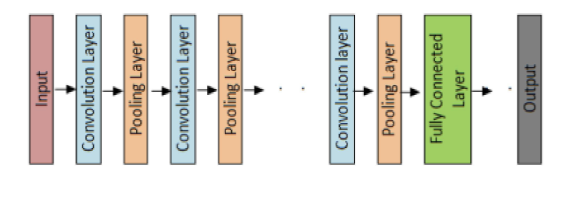
\includegraphics[width=\textwidth,height=0.65\textheight,keepaspectratio]{Figures/concepCNN.png}
            \caption{Feature hierarchy in a deep CNN}
        \end{figure}
    \end{columns}
\end{frame}

\begin{frame}{When to Use Transfer Learning - Recommended scenarios:}

    \begin{tabular}{lll}
        \toprule
        \textbf{Situation} & \textbf{Approach} & \textbf{Result} \\
        \midrule
        Small dataset, similar domain & Transfer + fine-tune last layers & Excellent \\
        Small dataset, different domain & Transfer + retrain more layers & Good \\
        Large dataset, similar domain & Fine-tune entire network & Very good \\
        Large dataset, different domain & Train from scratch & Possible \\
        \bottomrule
    \end{tabular}

    \begin{alertblock}{Most common case in practice:}
        Small dataset + domain related to ImageNet (objects, scenes, textures)
        $\Rightarrow$ \textbf{Transfer Learning is the go-to approach.}
    \end{alertblock}
\end{frame}

%================================================
\section{Transfer Learning Strategies}
%================================================

\begin{frame}{Two Main Strategies}
    \begin{columns}
        \column{0.5\textwidth}
        \begin{block}{1. Feature Extraction}
            \begin{itemize}
                \item \textbf{Freeze} all convolutional layers
                \item Only train the new classification head
                \item Fast, less data needed
                \item Risk: limited adaptation to new domain
            \end{itemize}
        \end{block}
        \column{0.5\textwidth}
        \begin{block}{2. Fine-Tuning}
            \begin{itemize}
                \item \textbf{Unfreeze} some or all layers
                \item Retrain with a \textbf{low learning rate}
                \item More flexible, better accuracy
                \item Risk: catastrophic forgetting if LR too high
            \end{itemize}
        \end{block}
    \end{columns}

    \begin{exampleblock}{Strategy used in Ex5:}
        \textbf{Fine-tuning of the last convolutional layer} (\texttt{conv10}) with high learning rate factors, while keeping all other layers at the pre-trained weights.
    \end{exampleblock}
\end{frame}

\begin{frame}{Transfer Learning vs. Training from Scratch}
    \begin{columns}
        \column{0.5\textwidth}
        \begin{alertblock}{Training from Scratch}
            \begin{itemize}
                \item Millions of samples required
                \item Days/weeks of training
                \item High risk of underfitting
                \item Justified only for very unique domains
            \end{itemize}
        \end{alertblock}
        \column{0.5\textwidth}
        \begin{block}{Transfer Learning}
            \begin{itemize}
                \item Hundreds of samples sufficient
                \item Minutes to hours of training
                \item High accuracy from the start
                \item Practical for most real problems
            \end{itemize}
        \end{block}
    \end{columns}
    \vspace{0.4cm}
    \begin{center}
        \textbf{Transfer Learning} has become the \textit{de facto} standard approach \\
        for applied deep learning with limited data.
    \end{center}
\end{frame}

\begin{frame}{Learning Rate Strategy in Fine-Tuning}
    The key to successful fine-tuning: \textbf{differential learning rates}.

    \begin{block}{Layer-wise Learning Rate Control}
        \begin{itemize}
            \item \textbf{Pre-trained layers}: very low LR (e.g., $\eta = 0.0001$) \\
                $\rightarrow$ Preserves general features already learned
            \item \textbf{New classification layers}: high LR factor (e.g., $\times 10$) \\
                $\rightarrow$ Adapts quickly to the new classes
        \end{itemize}
    \end{block}

    \begin{alertblock}{Catastrophic Forgetting}
        Using a high global learning rate will \textbf{destroy} the pre-trained weights. The network will "forget" what it learned on ImageNet, losing the advantage of transfer learning entirely.
    \end{alertblock}
\end{frame}

%================================================
\section{Pre-trained Networks in MATLAB}
%================================================

\begin{frame}{Available Pre-trained Networks}
    MATLAB's Deep Learning Toolbox includes a curated gallery of pre-trained CNNs:
    \begin{tabular}{lccl}
        \toprule
        \textbf{Network} & \textbf{Parameters} & \textbf{Input Size} & \textbf{Strength} \\
        \midrule
        SqueezeNet       & 1.24 M   & $227\times227$ & Compact, fast \\
        GoogLeNet        & 7 M      & $224\times224$ & Balanced \\
        ResNet-50        & 25 M     & $224\times224$ & High accuracy \\
        ResNet-101       & 44 M     & $224\times224$ & Very deep \\
        VGG-16           & 138 M    & $224\times224$ & Simple, powerful \\
        EfficientNet-b0  & 5.3 M    & $224\times224$ & Efficient scaling \\
        \bottomrule
    \end{tabular}

   
\end{frame}

\begin{frame}{SqueezeNet Architecture}
    \begin{columns}
        \column{0.55\textwidth}
        \textbf{SqueezeNet} (Iandola et al., 2016):
        \begin{itemize}
            \item Designed for \textbf{extreme compactness}
            \item Only \textbf{1.24 M parameters} (vs.\ 60 M in AlexNet)
            \item Comparable accuracy on ImageNet
            \item Key innovation: \textbf{Fire modules}
                \begin{itemize}
                    \item \textit{Squeeze}: $1\times1$ convolutions (dimensionality reduction)
                    \item \textit{Expand}: $1\times1$ + $3\times3$ convolutions
                \end{itemize}
            \item Final layer: \texttt{conv10} with 1000 filters
            \item Input size: $227 \times 227 \times 3$
        \end{itemize}
        \column{0.45\textwidth}
        \begin{block}{Why SqueezeNet for teaching?}
            \begin{itemize}
                \item No additional support package
                \item Trains on CPU in minutes
                \item Clear, inspectable architecture
                \item Ideal for small datasets
            \end{itemize}
        \end{block}
    \end{columns}
\end{frame}

\begin{frame}{SqueezeNet — Fire Module}
    \begin{block}{Fire Module Structure}
        Each Fire module consists of two stages:
        \quad \textbf{Squeeze} ($1\times1$ conv) $\longrightarrow$ \textbf{Expand} ($1\times1$ + $3\times3$ conv, concatenated)
    \end{block}

    \begin{columns}
        \column{0.5\textwidth}
        \begin{exampleblock}{Squeeze layer}
            \begin{itemize}
                \item Only $1\times1$ convolution filters
                \item Reduces the number of input channels (dimensionality compression)
                \item $9\times$ fewer parameters than a $3\times3$ filter
            \end{itemize}
        \end{exampleblock}
        \column{0.5\textwidth}
        \begin{exampleblock}{Expand layer}
            \begin{itemize}
                \item Mix of $1\times1$ and $3\times3$ convolution filters
                \item Outputs concatenated along the channel axis
                \item Recovers spatial information after squeeze
                \item Net result: $50\times$ fewer parameters vs.\ AlexNet
            \end{itemize}
        \end{exampleblock}
    \end{columns}
\end{frame}

%================================================
\section{Transfer Learning Pipeline in MATLAB}
%================================================

\begin{frame}{Complete Pipeline Overview}
    \begin{center}
    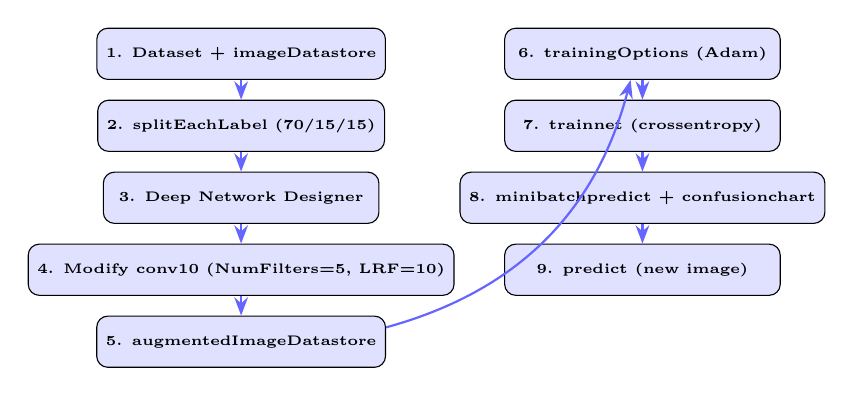
\begin{tikzpicture}[
        pstep/.style={rectangle, draw, rounded corners=4pt,
                     fill=blue!12, minimum width=3.5cm,
                     minimum height=0.65cm, font=\tiny\bfseries},
        arr/.style={-Stealth, thick, blue!60}
    ]
        \node[pstep] (ds)   {1. Dataset + imageDatastore};
        \node[pstep, below=0.25cm of ds]  (sp)   {2. splitEachLabel (70/15/15)};
        \node[pstep, below=0.25cm of sp]  (dnd)  {3. Deep Network Designer};
        \node[pstep, below=0.25cm of dnd] (mod)  {4. Modify conv10 (NumFilters=5, LRF=10)};
        \node[pstep, below=0.25cm of mod] (aug)  {5. augmentedImageDatastore};
        \node[pstep, right=1.5cm of ds]   (opt)  {6. trainingOptions (Adam)};
        \node[pstep, below=0.25cm of opt] (tr)   {7. trainnet (crossentropy)};
        \node[pstep, below=0.25cm of tr]  (ev)   {8. minibatchpredict + confusionchart};
        \node[pstep, below=0.25cm of ev]  (pr)   {9. predict (new image)};
        \draw[arr] (ds)--(sp); \draw[arr] (sp)--(dnd);
        \draw[arr] (dnd)--(mod); \draw[arr] (mod)--(aug);
        \draw[arr] (aug) to[bend right=30] (opt);
        \draw[arr] (opt)--(tr); \draw[arr] (tr)--(ev); \draw[arr] (ev)--(pr);
    \end{tikzpicture}
    \end{center}
\end{frame}

%------------------------------------------------
\subsection{Training}
%------------------------------------------------

\begin{frame}{The Adam Optimizer}
    \textbf{Adam} (\textit{Adaptive Moment Estimation}) maintains running estimates of first and second moments of the gradient:
    \begin{equation}
        m_t = \beta_1 m_{t-1} + (1-\beta_1)g_t
    \end{equation}
    \begin{equation}
        v_t = \beta_2 v_{t-1} + (1-\beta_2)g_t^2
    \end{equation}
    \begin{equation}
        \theta_{t+1} = \theta_t - \frac{\alpha}{\sqrt{\hat{v}_t} + \epsilon}\,\hat{m}_t
    \end{equation}
    \begin{itemize}
        \item $\hat{m}_t$, $\hat{v}_t$: bias-corrected estimates
        \item \textbf{Adaptive}: each parameter has its own effective LR
        \item \textbf{Robust} for small, heterogeneous datasets
        \item Default: $\beta_1=0.9$, $\beta_2=0.999$, $\epsilon=10^{-8}$
    \end{itemize}
\end{frame}

\begin{frame}[fragile]{Training Options}
\begin{lstlisting}[language=Matlab, style=MATLABStyle]
%% 4. OPCIONES DE ENTRENAMIENTO
options = trainingOptions("adam", ...
    InitialLearnRate=0.0001, ...        % Bajo: protege pesos preentrenados
    MaxEpochs=8, ...                    % Pocas epocas (TL converge rapido)
    ValidationData=imdsValidation, ...  % Monitor de sobreajuste
    ValidationFrequency=5, ...          % Valida cada 5 iteraciones
    MiniBatchSize=11, ...               % 52 imgs / 11 ~ 5 iter/epoca
    Plots="training-progress", ...      % Grafica perdida y precision
    Metrics="accuracy", ...
    Verbose=false);
\end{lstlisting}
\end{frame}
\begin{frame}[fragile]{Training Options}

    \begin{tabular}{lcl}
        \toprule
        \textbf{Option} & \textbf{Value} & \textbf{Justification} \\
        \midrule
        \texttt{InitialLearnRate} & 0.0001 & Protects pre-trained weights \\
        \texttt{MaxEpochs}        & 8      & Fast convergence in TL \\
        \texttt{MiniBatchSize}    & 11     & Even split of 52 training imgs \\
        \bottomrule
    \end{tabular}
\end{frame}

\begin{frame}{Cross-Entropy Loss Function}
    \texttt{trainnet} uses \textbf{categorical cross-entropy} as the loss function:
    \begin{equation}
        \mathcal{L} = -\sum_{i=1}^{C} y_i \log(\hat{y}_i)
    \end{equation}
    \begin{itemize}
        \item $C$: number of classes (5 in our example)
        \item $y_i$: true label (one-hot encoded: 1 for correct class, 0 otherwise)
        \item $\hat{y}_i$: predicted probability for class $i$ (output of softmax)
        \item Penalizes the network more when it is \textbf{confident and wrong}
    \end{itemize}
    
\end{frame}


%================================================
\section{Analysis and Reflection}
%================================================

\begin{frame}{Hyperparameter Sensitivity Analysis}
    \begin{tabular}{lll}
        \toprule
        \footnotesize
        \textbf{Change} & \textbf{Effect} & \textbf{Why} \\
        \midrule
        $\uparrow$ \texttt{MaxEpochs} (e.g., 20) & Overfitting & Memorizes training data \\
        $\uparrow$ \texttt{InitialLearnRate} (0.01) & Catastrophic forgetting & Destroys pre-trained weights \\
        $\downarrow$ \texttt{WeightLearnRateFactor} (1) & Slower adaptation & \texttt{conv10} learns too slowly \\
        Remove augmentation & More overfitting & Fewer effective training samples \\
        Use ResNet-50 instead & Higher accuracy & More parameters, richer features \\
        \bottomrule
    \end{tabular}
    \vspace{0.3cm}
    \begin{exampleblock}{Try with MATLAB Experiment Manager:}
        The \textbf{Experiment Manager} app runs multiple hyperparameter configurations in parallel and plots comparison curves automatically.
    \end{exampleblock}
\end{frame}

\begin{frame}{Questions for Reflection}
    \begin{enumerate}
        \item What happens if you increase \texttt{MaxEpochs} to 20? How does the training/validation gap evolve?

        \vspace{0.3cm}
        \item What happens if \texttt{InitialLearnRate} is set to 0.01? What does this tell us about catastrophic forgetting?

        \vspace{0.3cm}
        \item What would be the effect of setting \texttt{WeightLearnRateFactor = 1} in \texttt{conv10}?

        \vspace{0.3cm}
        \item Which pre-trained network would give better results on this dataset? Justify your answer in terms of parameters, depth, and input size.

        \vspace{0.3cm}
        \item How does the confusion matrix change with and without data augmentation? What does this tell us about the role of regularization in Transfer Learning?
    \end{enumerate}
\end{frame}

\begin{frame}{Key Concepts — Reference Table}
    \begin{adjustbox}{max width=\textwidth}
    \begin{tabular}{lll}
        \toprule
        \textbf{Concept} & \textbf{Meaning} & \textbf{In Ex5} \\
        \midrule
        Transfer Learning   & Reuse weights from a source task & SqueezeNet (ImageNet) $\to$ 5 classes \\
        Fine-tuning         & Selective retraining of final layers & Only \texttt{conv10} modified aggressively \\
        \texttt{imageDatastore} & Efficient image container (batch I/O) & Reads 75 images without RAM overload \\
        Data Augmentation   & Artificial training variants & Flip + $\pm30$px translations \\
        Adam                & Adaptive gradient optimizer & Converges well on small datasets \\
        Cross-entropy loss  & Classification loss function & Measures predicted vs.\ true distribution \\
        Confusion matrix    & Per-class error visualization & Identifies class-specific confusions \\
        \texttt{minibatchpredict} & Batch prediction (efficient) & Classifies test set in batches \\
        \texttt{scores2label}    & Scores $\to$ class labels (argmax) & Converts probabilities to class names \\
        \bottomrule
    \end{tabular}
    \end{adjustbox}
\end{frame}

%================================================
\section{Summary}
%================================================

\begin{frame}{Summary}
    \begin{columns}
        \column{0.5\textwidth}
        \textbf{What we covered:}
        \begin{itemize}
            \item Why training from scratch is impractical for small datasets
            \item How CNNs learn hierarchical features that generalize
            \item Feature Extraction vs.\ Fine-Tuning strategies
            \item Pre-trained networks available in MATLAB
            \item SqueezeNet architecture and Fire modules
            \item Full pipeline: data $\to$ train $\to$ evaluate $\to$ predict
        \end{itemize}
        \column{0.5\textwidth}
        \textbf{Key takeaways:}
        \begin{block}{Transfer Learning in practice}
            \begin{itemize}
                \item \textbf{Low LR} for pre-trained layers
                \item \textbf{High LR factor} for new classification head
                \item \textbf{Data augmentation} is essential with small datasets
                \item \textbf{Confusion matrix} $>$ global accuracy for diagnosis
                \item Deep Network Designer enables GUI-based TL without code
            \end{itemize}
        \end{block}
    \end{columns}
\end{frame}

\begin{frame}{References and Further Reading}
    \begin{exampleblock}{MathWorks Documentation}
        \begin{itemize}
            \item \url{https://la.mathworks.com/discovery/transfer-learning.html}
            \item \url{https://la.mathworks.com/help/deeplearning/ug/transfer-learning-with-deep-network-designer.html}
        \end{itemize}
    \end{exampleblock}
    \begin{block}{Key Papers}
        \begin{itemize}
            \item Iandola et al.\ (2016) — \textit{SqueezeNet: AlexNet-level accuracy with 50x fewer parameters}
            \item Pan \& Yang (2010) — \textit{A Survey on Transfer Learning}, IEEE TKDE
            \item Yosinski et al.\ (2014) — \textit{How transferable are features in deep neural networks?}
            \item Kornblith et al.\ (2019) — \textit{Do Better ImageNet Models Transfer Better?}
        \end{itemize}
    \end{block}
    \begin{center}
        \large\textbf{Example: Ex5\_KnowledgeTransfer} \\
        \small\texttt{/Examples/Ex5\_KnowledgeTransfer/Ex5.m}
    \end{center}
\end{frame}

\end{document}
